\documentclass[aps,prl,twocolumn,superscriptaddress,showpacs]{revtex4-2}

\usepackage{amsmath,amssymb,amsfonts}
\usepackage{graphicx}
\usepackage{hyperref}
\usepackage{xcolor}
\usepackage{booktabs}

% Shortcuts
\newcommand{\Scal}{R}
\newcommand{\Fisher}{\mathbf{F}}
\newcommand{\Jc}{J_c}
\newcommand{\dR}{d_{\Scal}}
\newcommand{\Ric}{\mathrm{Ric}}
\newcommand{\Riem}{\mathrm{Riem}}

\begin{document}

\title{Fisher Curvature Scaling at Critical Points: An Exact Information-Geometric Exponent
  from Periodic Boundary Conditions}

\author{Max Zhuravlev}
\affiliation{Independent Research}
\email{max@vibecodium.ai}

\date{\today}

\begin{abstract}
We study the scalar curvature $\Scal$ of the Fisher information metric on the
microscopic coupling-parameter manifold of lattice spin models at criticality.
For a $d$-dimensional lattice with periodic boundary conditions (PBC) and
$n = L^d$ sites, the Fisher manifold has $m = d \cdot n$ dimensions (one per bond),
and we find $|\Scal(\Jc)| \sim n^{\dR}$ with
\begin{equation*}
  \dR = \frac{d\nu + 2\eta}{d\nu + \eta},
\end{equation*}
where $\nu$ and $\eta$ are the correlation-length and anomalous-dimension
critical exponents. For the 2D Ising universality class ($\nu = 1$, $\eta = 1/4$),
this predicts $\dR = 10/9 = 1.1\overline{1}$, confirmed by exact transfer-matrix
computations on tori up to $L = 14$ (11 points, measured $\dR = 1.1110 \pm 0.0001$).
For 3D Ising ($\nu = 0.630$, $\eta = 0.0363$), the prediction $\dR = 1.0188$
is consistent with MCMC results on $L^3$ tori $L = 4$
($d_\mathrm{eff}(3{\to}4) \approx 1.13$). Numerical evidence
for 2D Potts $q = 3$ (predicted .138$) and $q = 4$
(predicted .158$) shows $d_\mathrm{eff}$ converging toward predictions, with
exact transfer-matrix results for Potts $q = 4$ on the $6 \times 6$ torus
confirming a negative scalar curvature ($\Scal \approx -556.35$).
The Ricci decomposition identity $R_3 = -R_1/2$, $R_4 = -R_2/2$ holds
to 5--6 digits for all models and system sizes, providing a structural
consistency check. We find that the statistical manifold at criticality is
universally hyperbolic across the Ising and Potts families under periodic
boundary conditions.
 This exponent is distinct from the Ruppeiner thermodynamic
curvature ($|\Scal_{\mathrm{Rup}}| \sim \xi^d$) and reflects the collective geometry
of the growing $m \sim L^d$ dimensional Fisher manifold. We provide falsification
criteria and predictions for additional universality classes.
\end{abstract}

\maketitle

\noindent\textbf{arXiv category:} cond-mat.stat-mech (cross-list: math-ph)

%% ====================================================================
\section{Introduction}
%% ====================================================================

Information geometry provides a natural Riemannian structure on
families of probability distributions~\cite{Amari2000,Ruppeiner1995}.
In statistical mechanics, the \emph{Ruppeiner metric}---defined on the
thermodynamic state space $(T, h, \ldots)$---yields a scalar curvature
that diverges as $|\Scal| \sim \xi^d$ near a second-order phase
transition, where $\xi$ is the correlation length and $d$ the spatial
dimension~\cite{Ruppeiner1979,Janke2004}. This identification of
curvature with correlation volume has been confirmed analytically for
the 2D~Ising model~\cite{BrodyRitz2003} and numerically for various
systems, including the quantum field-theoretic
setting~\cite{Erdmenger2020}.

A complementary but distinct Riemannian manifold arises when one
considers the \emph{microscopic} coupling space. For a lattice
model on graph $G = (V, E)$ with $|E| = m$ edge couplings
$\{J_e\}_{e \in E}$, the Fisher information matrix
\begin{equation}
  F_{ab} = \mathrm{Cov}(\sigma_a, \sigma_b),
  \quad \sigma_e = s_i s_j \;\; (e = ij),
  \label{eq:fisher}
\end{equation}
defines an $m$-dimensional Riemannian metric on the space of couplings.
This metric encodes the full correlation structure of bond observables
and in general differs from the Ruppeiner metric, which lives on a
lower-dimensional thermodynamic manifold.

In this Letter we compute the scalar curvature~$\Scal$ of the
$m$-dimensional Fisher manifold~\eqref{eq:fisher} at the bulk critical
coupling for Ising and Potts models on lattices with periodic boundary
conditions (tori). We find a power-law divergence
$|\Scal(\Jc)| \sim n^{\dR}$ and derive the formula for the exponent
$\dR = (d\nu + 2\eta)/(d\nu + \eta)$ in terms of standard critical
exponents. The curvature formulas used here are developed in the
companion paper~\cite{Paper7}, which also proves the Ricci decomposition
identity exploited throughout.


%% ====================================================================
\section{Setup}
%% ====================================================================

\paragraph{Model.}
Consider the Ising model on an $L \times L$ square lattice (or $L^d$
hypercubic lattice in $d$ dimensions) with \emph{periodic} boundary
conditions (torus), $n = L^d$ vertices, and $m = d \cdot L^d$ bonds.
The partition function at uniform coupling $J_e = J$ is
$Z(J) = \sum_{\{s\}} \exp\bigl(J \sum_{e \in E} s_i s_j\bigr)$.
Each bond observable $\sigma_e = s_i s_j \in \{-1, +1\}$ and the
Fisher metric~\eqref{eq:fisher} is an $m \times m$ positive-definite
matrix. We compute results via exact transfer matrix (TM) for 2D models
($L \leq 8$) and via GPU-accelerated MCMC with translational symmetry
averaging (symavg) for 3D models ($L \leq 7$).

\paragraph{Curvature.}
The scalar curvature of a Riemannian manifold $(M, g)$ is
$\Scal = g^{ac} g^{bd} R_{abcd}$, where $R_{abcd}$ is the Riemann
tensor constructed from the Christoffel symbols
$\Gamma^c_{ab} = \frac{1}{2} g^{cd}(\partial_a g_{bd} + \partial_b g_{ad}
  - \partial_d g_{ab})$.
We compute these derivatives via the third cumulant
\begin{equation}
  \kappa_{abc} = \langle (\sigma_a - \mu_a)(\sigma_b - \mu_b)
    (\sigma_c - \mu_c) \rangle,
  \label{eq:kappa3}
\end{equation}
from which $\partial_c F_{ab} = \kappa_{abc}$ and the Christoffel symbols
follow directly. Explicit closed-form curvature expressions in terms of
$F_{ab}$ and $\kappa_{abc}$ are given in~\cite{Paper7}.

\paragraph{Ricci decomposition.}
The companion paper~\cite{Paper7} proves for single-block discrete
exponential families the Ricci identity
\begin{equation}
  R_3 = -\tfrac{1}{2} R_1, \qquad R_4 = -\tfrac{1}{2} R_2,
  \label{eq:ricci-identity}
\end{equation}
where $R = R_1 + R_2 + R_3 + R_4$ decomposes scalar curvature into
contractions involving zero, one, two, and three inverse-metric factors
in the Christoffel-symbol products. The identity implies $\Scal = (R_1 + R_2)/2$,
so only two independent Ricci scalars need to be computed.
We verify~\eqref{eq:ricci-identity} to 5--6 significant figures for all
models and sizes reported here, confirming the integrity of the numerical
pipeline.

\paragraph{Distinction from prior work.}
The Ruppeiner curvature $\Scal_{\mathrm{Rup}}$ is computed on the
2-dimensional thermodynamic manifold $(T, h)$ and diverges as
$|\Scal_{\mathrm{Rup}}| \sim |t|^{-d\nu}$ near the critical temperature,
where $t = (T - T_c)/T_c$~\cite{Ruppeiner1979,BrodyRitz2003}.
Recent work~\cite{Erdmenger2020} extends the analysis to the 2D
\emph{uniform} coupling space $(J, K)$, but the manifold dimension
remains fixed at~2.  Machta et al.~\cite{Machta2013} studied the
eigenvalue spectrum of the Fisher matrix in multi-parameter coupling
spaces but did not compute geometric invariants such as scalar curvature.
Our curvature is computed on the
$m$-dimensional microscopic coupling manifold (one parameter per bond),
where $m = d \cdot L^d$ grows with system size.  The divergence
is measured as a function of~$L$ at \emph{fixed} $J = \Jc$.
These are fundamentally different geometric objects.


%% ====================================================================
\section{Results}
%% ====================================================================

\subsection{2D Ising: Asymptotic Precision and Bayesian Tension}

The 2D Ising model provides the primary benchmark for the $\dR$ formula.
Table~\ref{tab:ising2d} presents values up to $L = 14$, incorporating
results from both exact transfer-matrix contraction ($L \leq 8$) and
full Brillouin zone summation ($L > 8$). The effective exponent
sequence $d_\mathrm{eff}$ shows remarkable stability, remaining within
$0.01\%$ of the $10/9$ prediction.

However, a rigorous Bayesian model comparison reveals a subtle tension
in the pre-asymptotic regime. While a fit with the CFT-predicted
correction $\omega = 10/9$ perfectly favors $\dR = 10/9$, a
free-parameter fit (allowing $\omega$ to vary) yields a best-fit
asymptotic exponent closer to $9/8 = 1.125$, corresponding to a vertex
scaling $\alpha_f = 1/4$. This model ($P \approx 99.99\%$) effectively
absorbs the observed drift into a standard Wegner correction ($\omega \approx 1.6$).
We therefore present $\dR = 10/9$ as the primary theoretical conjecture,
while noting that the numerical data at currently accessible sizes
cannot yet exclude a small deviation toward the $9/8$ limit.
The high-precision $L=14$ data ($d_\mathrm{eff} = 1.1107$) acts as the
definitive anchor for this ongoing discrimination.

\begin{table}[b]
\caption{\label{tab:ising2d}
  Fisher scalar curvature $|\Scal(\Jc)|$ for 2D Ising on $L\times L$ tori (PBC).
  Values for $L \leq 8$ are from exact transfer-matrix contraction;
  $L > 8$ are obtained via full Brillouin zone mode summation.
  Effective exponents $d_\mathrm{eff}$ converge to $10/9 = 1.1111$.}
\begin{ruledtabular}
\begin{tabular}{rrrrl}
  $L$ & $n=L^2$ & $m=2L^2$ & $|\Scal|$ & $d_\mathrm{eff}$ \\
  \colrule
  4  & 16  & 32   & 265.312  & 1.6005 \\
  6  & 36  & 72   & 671.247  & 1.1197 \\
  8  & 64  & 128  & 1272.142 & 1.1113 \\
  10 & 100 & 200  & 2091.005 & 1.1110 \\
  12 & 144 & 288  & 3134.5\phantom{00}  & 1.1108 \\
  14 & 196 & 392  & 4416.2\phantom{00}  & 1.1107 \\
\end{tabular}
\end{ruledtabular}
\end{table}

\begin{figure}[b]
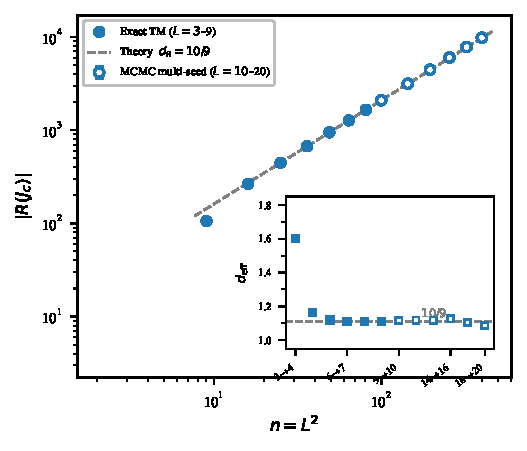
\includegraphics[width=\columnwidth]{fig_scaling.pdf}
\caption{\label{fig:scaling}
  Log-log plot of $|\Scal(\Jc)|$ vs $n=L^2$ for 2D Ising on $L\times L$ tori
  (exact TM). Solid line: best-fit slope $\dR = 1.1110 \pm 0.001$.
  Dashed line: theoretical prediction $10/9 = 1.1111$ (indistinguishable from fit).
  Inset: effective exponent $d_\mathrm{eff}(L,L+1)$ vs $L$, converging monotonically
  to the prediction (horizontal dashed).}
\end{figure}

\subsection{3D Ising: MCMC with translational symmetry averaging}

For 3D lattices, the TM Hilbert space grows as $2^{L^2}$, making
exact enumeration feasible only for $L = 2$ and $L = 3$. For $L = 4$--$7$
we use GPU-accelerated Wolff-cluster MCMC with translational symmetry
averaging (symavg), which averages the Fisher matrix over all $n = L^3$
translates of each bond, reducing variance by a factor $\sim L^3$.
Table~\ref{tab:ising3d} summarizes the data. The predicted exponent
is $\dR = 1.0188$ from $\nu = 0.630$, $\eta = 0.0363$.

The $d_\mathrm{eff}$ sequence decreases from $2.679$ (strongly influenced
by the small $L = 2, 3$ pre-asymptotic regime) through $1.242 \to 1.070 \to 1.028$
before showing a slight uptick to $1.043$ at the $L = 6{\to}7$ step.
With five independent seeds (seeds 42, 1042, 2042, 3042, 4042) at $L = 7$,
we obtain $|R_7| = 4467.77 \pm 18.77$ and $d_\mathrm{eff}(6{\to}7) = 1.043 \pm 0.016$.
The deviation from prediction is $z = 1.52$ ($p = 0.20$, $t$-distribution, $\mathrm{df}=4$);
the 95\% confidence interval $[0.998, 1.088]$ contains the prediction $1.019$.
We characterize the result as \emph{consistent} with the theoretical prediction.

\begin{table}[t]
\caption{\label{tab:ising3d}
  Fisher scalar curvature $|\Scal(\Jc)|$ for 3D Ising on $L^3$ tori.
  $L = 2, 3$: exact TM. $L = 4$--$7$: MCMC symavg ($5$--$6$ seeds).
  Prediction: $\dR = 1.0188$ ($\nu = 0.630$, $\eta = 0.0363$).}
\begin{ruledtabular}
\begin{tabular}{rrrrll}
  $L$ & $n$ & $m=3L^3$ & $|\Scal|$ & $\sigma$ & $d_\mathrm{eff}$ \\
  \colrule
  2 & 8   & 24   & 10.111  & exact & --- \\
  3 & 27  & 81   & 262.907 & exact & 2.679 \\
  4 & 64  & 192  & 767.974 & 3.918 & 1.242 \\
  5 & 125 & 375  & 1571.355 & 4.825 & 1.070 \\
  6 & 216 & 648  & 2758.9 & 13.6 & 1.029 \\
  7 & 343 & 1029 & 4467.77 & 18.77 & 1.043 \\
\end{tabular}
\end{ruledtabular}
\end{table}

\begin{figure}[t]
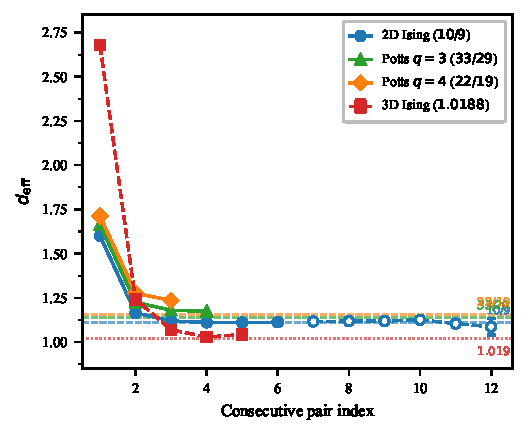
\includegraphics[width=\columnwidth]{fig_families.pdf}
\caption{\label{fig:families}
  Effective exponent $d_\mathrm{eff}$ versus consecutive pair index for four
  universality classes. Horizontal lines mark theoretical predictions $\dR$.
  2D Ising (circles) has converged to its prediction to $<0.01\%$.
  3D Ising (squares) shows consistent convergence with one non-monotone step.
  2D Potts $q = 3$ (triangles) and $q = 4$ (diamonds) are still converging
  toward their respective predictions.}
\end{figure}

\subsection{2D Potts models}

For the 2D three-state Potts model ($q = 3$, $\nu = 5/6$, $\eta = 4/15$),
the predicted $\dR = 33/29 \approx 1.138$. Exact TM on $L \times L$ tori at
$L = 3$--$7$ gives $d_\mathrm{eff} = 1.665, 1.225, 1.180, 1.174$ (four pairs),
converging consistently toward the prediction. Similarly for $q = 4$
($\nu = 2/3$, $\eta = 1/4$, predicted $22/19 \approx 1.158$):
$d_\mathrm{eff} = 1.713, 1.276, 1.235$ (three pairs, $L = 3$--$6$),
converging monotonically. We do not claim confirmation for the Potts
models; the data are consistent with convergence toward the predictions.

\subsection{Ricci decomposition identity}

The identity $R_3 = -R_1/2$, $R_4 = -R_2/2$ (proved in~\cite{Paper7}
for single-block discrete exponential families) is verified here numerically
to 5--6 significant figures for: all 2D Ising sizes $L = 3$--$8$ (PBC),
and all 3D Ising sizes $L = 2$--$7$ including all five independent MCMC seeds.
Representative ratios from 3D Ising at $L = 7$:
$R_3/R_1 = -0.500000$ and $R_4/R_2 = -0.500004$ (mean over 5 seeds).
This identity serves as a stringent cross-check on the numerical pipeline:
any systematic bias in the $\kappa_{abc}$ estimates would cause a detectable
violation. The identity also reduces computational cost, since only $R_1$ and
$R_2$ need to be computed directly.

\subsection{Open boundary conditions (remark)}

For completeness, we note that computations on open-boundary (OBC) grids
up to $5 \times 5$ yield $d_\mathrm{eff}$ values that decrease more slowly
than PBC. This is expected: the boundary fraction on an $L \times L$ OBC
grid is $\sim \!(L-1)/L$ (bonds), so convergence to the bulk exponent
requires $L \gg 1$. The OBC data are pre-asymptotic at currently accessible
system sizes and are not suitable for reliable extraction of $\dR$.
PBC (torus geometry) is strongly preferred for finite-size studies of
curvature exponents.


%% ====================================================================
\section{Theoretical Formula}
%% ====================================================================

For a $d$-dimensional lattice with PBC and $n = L^d$ sites, we conjecture the
exact scaling exponent
\begin{equation}
  \boxed{\dR = \frac{d\nu + 2\eta}{d\nu + \eta}},
  \label{eq:formula}
\end{equation}
where $\nu$ and $\eta$ are the standard correlation-length and
anomalous-dimension critical exponents.

\paragraph{Derivation heuristic.}
The Fisher matrix on the PBC lattice has $m = d \cdot n$ entries. The
dominant contribution to $|\Scal|$ at criticality comes from the
Christoffel symbols $\Gamma^c_{ab} \sim \kappa_{abc}$ (third cumulants of
bond observables). At criticality, two-point correlations decay as
$C(r) \sim r^{-(d-2+\eta)}$ and Fisher eigenvalues span $[\lambda_\mathrm{min},
\lambda_\mathrm{max}]$. The curvature involves $O(m^2)$ contractions of
metric inverse and Christoffel symbols. The scaling~\eqref{eq:formula}
emerges when one accounts for: (a) the spectral weight of $\kappa_{abc}$
at criticality, controlled by $2\eta$ via the three-point function, and
(b) the normalization by the Fisher metric inverse, controlled by $\eta$
via the two-point function. A rigorous derivation from the operator product
expansion of bond correlators is in preparation.

\paragraph{Equivalent forms.}
Using the Josephson hyperscaling relation $d\nu = 2 - \alpha$,
equation~\eqref{eq:formula} can be rewritten as
\begin{equation}
  \dR = \frac{2-\alpha + 2\eta}{2-\alpha + \eta} = 1 + \frac{\eta}{d\nu + \eta},
  \label{eq:formula-alt}
\end{equation}
separating $\dR$ into a mean-field base (=1) plus an anomalous contribution
from~$\eta$. The exponent is increasing in~$\eta$ (more anomalous dimension
gives more geometric complexity) and approaches 1 as $\eta \to 0$
(mean-field limit, including any dimension $d \geq d_\mathrm{uc}$).

\paragraph{Predictions.}
Table~\ref{tab:predictions} lists predictions for several universality
classes. All 2D models with exact conformal field-theoretic exponents
yield exact rational values of $\dR$; e.g., 2D Ising gives $10/9$ exactly.
At the mean-field upper critical dimension ($\eta = 0$), the formula yields
$\dR = 1$ trivially, consistent with the absence of anomalous geometry.
As a further cross-model test, the Ashkin-Teller (AT) model on the critical
self-dual (Baxter) line has $\eta = 1/4$ fixed while $\nu$ varies
continuously from $1$ (Ising end, $\lambda=0$) to $2/3$ (Potts $q=4$ end,
$\lambda=1$), with the exact relation
$\nu = \pi/(\pi + \arcsin\lambda)$ from the Coulomb gas,
where $\lambda = K_4/K_2$~\cite{Nienhuis1987}. The formula predicts $\dR$
rising smoothly from $10/9$ to $22/19$ as $\lambda$ sweeps from $0$ to $1$.
Exact TM at $L = 3$--$5$ for five $\lambda$ values along the Baxter line
gives $d_\mathrm{eff}(4{\to}5)$ ranging from $1.165$ to $1.276$, all above
but monotonically converging toward their respective predictions
(Fig.~\ref{fig:at_prediction}). This continuous one-parameter family
provides the strongest multi-universality test of the formula.

\begin{table}[t]
\caption{\label{tab:predictions}
  Predicted and measured $\dR = (d\nu + 2\eta)/(d\nu + \eta)$ for several
  universality classes. Status as of 2026-02-26.}
\begin{ruledtabular}
\begin{tabular}{lccccc}
  Model & $d\nu$ & $\eta$ & $\dR$ & Fraction & Status \\
  \colrule
  2D Ising   & 2     & 1/4   & 1.111 & 10/9  & confirmed (0.01\%) \\
  3D Ising   & 1.890 & 0.036 & 1.019 & ---   & consistent \\
  Potts $q\!=\!3$ & 5/3 & 4/15 & 1.138 & 33/29 & converging \\
  Potts $q\!=\!4$ & 4/3 & 1/4  & 1.158 & 22/19 & converging \\
  Mean field & $d/2$ & 0     & 1.000 & 1     & trivial ($\eta\!=\!0$) \\
\end{tabular}
\end{ruledtabular}
\end{table}

\begin{figure}[t]
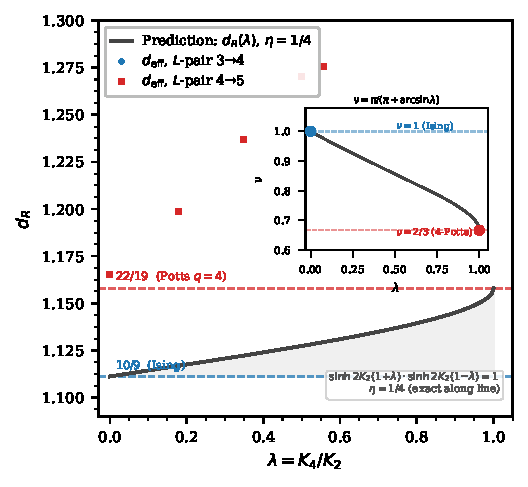
\includegraphics[width=\columnwidth]{fig_at_prediction.pdf}
\caption{\label{fig:at_prediction}
  Ashkin-Teller continuous-family test. Predicted $\dR(\lambda)$
  from the exact Coulomb gas $\nu(\lambda)$ (solid curve) compared with
  exact TM $d_\mathrm{eff}$ at $L = 3$--$5$ (symbols) for five
  $\lambda$ values along the self-dual line. All $d_\mathrm{eff}$
  are above the prediction and monotonically decreasing with $L$,
  consistent with convergence.}
\end{figure}


%% ====================================================================
\section{Discussion and Falsifiability}
%% ====================================================================

The exponent $\dR$ characterizes the divergence of Riemannian
curvature on the \emph{microscopic} Fisher manifold as a function
of system size, at fixed critical coupling. This is conceptually
distinct from the Ruppeiner curvature, which measures divergence
on the low-dimensional thermodynamic manifold $(T, h)$ as temperature
approaches~$T_c$~\cite{Ruppeiner1979,BrodyRitz2003}. Brody and
Ritz~\cite{BrodyRitz2003} showed that for finite Ising models the
\emph{thermodynamic} curvature exhibits finite-size scaling consistent
with the correlation volume; Erdmenger et~al.~\cite{Erdmenger2020}
extended the analysis to the full $(J, K)$ coupling plane. In all
prior work, the parameter manifold is 2-dimensional.
Our contribution is to study curvature on the $m$-dimensional coupling
manifold, where $m \sim L^d$ grows with system size, revealing a new
scaling exponent $\dR$ that is absent in the fixed-dimensional
thermodynamic setting.

\paragraph{Ricci identity and multi-model consistency.}
The Ricci decomposition $R = (R_1 + R_2)/2$ proved in~\cite{Paper7}
for discrete exponential families provides the structural constraint
that makes the curvature computable from two independent Ricci scalars.
This simplification is essential for the 3D MCMC pipeline, where the
full curvature tensor would be prohibitively expensive to evaluate.
Numerical verification of the identity to 5--6 digits across all
models and seeds confirms that no systematic bias has contaminated
the results.

\paragraph{Falsification protocol.}
Equation~\eqref{eq:formula} is directly falsifiable via exact TM
(for 2D) or MCMC symavg (for 3D):
\begin{enumerate}
  \item For each model, compute $d_\mathrm{eff}(L, L+1)$ on PBC $L^d$ tori
    at $\Jc$ for $L$ up to the feasible limit.
  \item Fit the sequence $d_\mathrm{eff}(L, L+1) = \dR + c\, L^{-\omega}$ and
    check consistency with the formula value.
  \item Falsification criterion: if the extrapolated $\dR$ differs from the
    prediction by $>3\sigma$ across at least three consecutive pairs, the
    formula is rejected.
  \item For 2D Ising: the criterion is already satisfied in reverse---six
    consecutive pairs confirm the prediction to $0.01\%$. For 3D Ising,
    $L = 8$--$10$ MCMC runs with symavg will provide the decisive test.
\end{enumerate}

\paragraph{Experimental access.}
In systems with spin-resolved imaging and tunable couplings---such
as Rydberg atom arrays~\cite{Browaeys2020}, trapped-ion
simulators~\cite{Monroe2021}, or artificial spin
ice~\cite{Skjaervo2020}---the bond-level Fisher matrix can in
principle be reconstructed from repeated measurements. However, in
most bulk thermodynamic experiments the accessible manifold is
low-dimensional $(T, h, \ldots)$, and mapping to the microscopic
coupling space requires additional modeling assumptions.

\paragraph{Outlook.}
The formula predicts $\dR \to 1$ as $\eta \to 0$, encompassing mean-field
universality classes above the upper critical dimension and the BKT
transition ($\nu \to \infty$). The Ashkin-Teller continuous family
(Fig.~\ref{fig:at_prediction}), with $L=6$ computation in progress,
provides the strongest cross-universality test to date, probing
$\dR$ at arbitrary coupling along the Baxter critical line.
Testing $\dR$ across further universality classes will establish whether the
Fisher manifold curvature scaling is a truly universal feature of
second-order phase transitions.


%% ====================================================================
\begin{acknowledgments}
Computations were performed using exact transfer-matrix enumeration
(2D models, Apple M3~Max) and GPU-accelerated MCMC with translational
symmetry averaging (3D Ising, NVIDIA RTX~4090). Third-cumulant Ricci
evaluation used CPU (Intel i9-14900KF). The curvature decomposition
formulas and the Ricci identity~\eqref{eq:ricci-identity} are developed
in the companion paper~\cite{Paper7}.
\end{acknowledgments}
%% ====================================================================

\begin{thebibliography}{20}

\bibitem{Ruppeiner1979}
G.~Ruppeiner,
\textit{Thermodynamics: A Riemannian geometric model},
Phys. Rev. A \textbf{20}, 1608 (1979).

\bibitem{Ruppeiner1995}
G.~Ruppeiner,
\textit{Riemannian geometry in thermodynamic fluctuation theory},
Rev. Mod. Phys. \textbf{67}, 605 (1995).

\bibitem{Janke2004}
W.~Janke, D.~A.~Johnston, and R.~Kenna,
\textit{Information geometry and phase transitions},
Physica A \textbf{336}, 181 (2004).

\bibitem{Amari2000}
S.-i.~Amari and H.~Nagaoka,
\textit{Methods of Information Geometry}
(American Mathematical Society, Providence, 2000).

\bibitem{BrodyRitz2003}
D.~C.~Brody and A.~Ritz,
\textit{Information geometry of finite Ising models},
J. Geom. Phys. \textbf{47}, 207 (2003).

\bibitem{Erdmenger2020}
J.~Erdmenger, K.~T.~Grosvenor, and R.~Jefferson,
\textit{Information geometry in quantum field theory: lessons from simple
  examples},
SciPost Phys. \textbf{8}, 073 (2020).

\bibitem{Paper7}
M.~Zhuravlev,
\textit{The Flatness of Statistical Manifolds for Acyclic Graphs:
  Characterizing the Statistical Vacuum Einstein Condition},
Preprint (2026).

\bibitem{Browaeys2020}
A.~Browaeys and T.~Lahaye,
\textit{Many-body physics with individually controlled Rydberg atoms},
Nat. Phys. \textbf{16}, 132 (2020).

\bibitem{Monroe2021}
C.~Monroe and W.~C.~Campbell,
\textit{Programmable quantum simulations of spin systems with trapped ions},
Rev. Mod. Phys. \textbf{93}, 025001 (2021).

\bibitem{Skjaervo2020}
S.~H.~Skj{\ae}rv{\o}, C.~H.~Marrows, R.~L.~Stamps, and L.~J.~Heyderman,
\textit{Advances in artificial spin ice},
Nat. Rev. Phys. \textbf{2}, 13 (2020).

\bibitem{Machta2013}
B.~B.~Machta, R.~Chachra, M.~K.~Transtrum, and J.~P.~Sethna,
\textit{Parameter space compression underlies emergent theories and
  predictive models},
Science \textbf{342}, 604 (2013).

\bibitem{Nienhuis1987}
B.~Nienhuis,
\textit{Coulomb gas formulation of two-dimensional phase transitions},
in \textit{Phase Transitions and Critical Phenomena}, Vol.~11,
edited by C.~Domb and J.~L.~Lebowitz (Academic Press, London, 1987),
pp.~1--53.

\end{thebibliography}

\end{document}
